% =============================================================================
% Section 4.5: Media and Video Processing Module
% =============================================================================

\section{Media and Video Processing Module}
\label{sec:media-module}

\subsection{Functional Description}

The Media module manages the full lifecycle of video assets from upload to delivery. It integrates with Mux (Section~\ref{sec:video-streaming}) for transcoding, storage, and CDN delivery, while maintaining its own domain model for asset state and metadata. The module provides REST endpoints for creating direct upload URLs, querying asset status, and generating signed playback tokens for enrolled learners.

The module interacts closely with the AI Pipeline module (Section~\ref{sec:ai-pipeline-module}): when a video reaches the READY state, the Media module publishes a \texttt{VideoReady} event that triggers automatic transcript generation.

\subsection{Mux Integration and VideoAsset State Machine}

The \texttt{VideoAsset} aggregate root tracks the lifecycle of each uploaded video through the states illustrated in Figure~\ref{fig:video-statemachine}.

\begin{figure}[H]
  \centering
  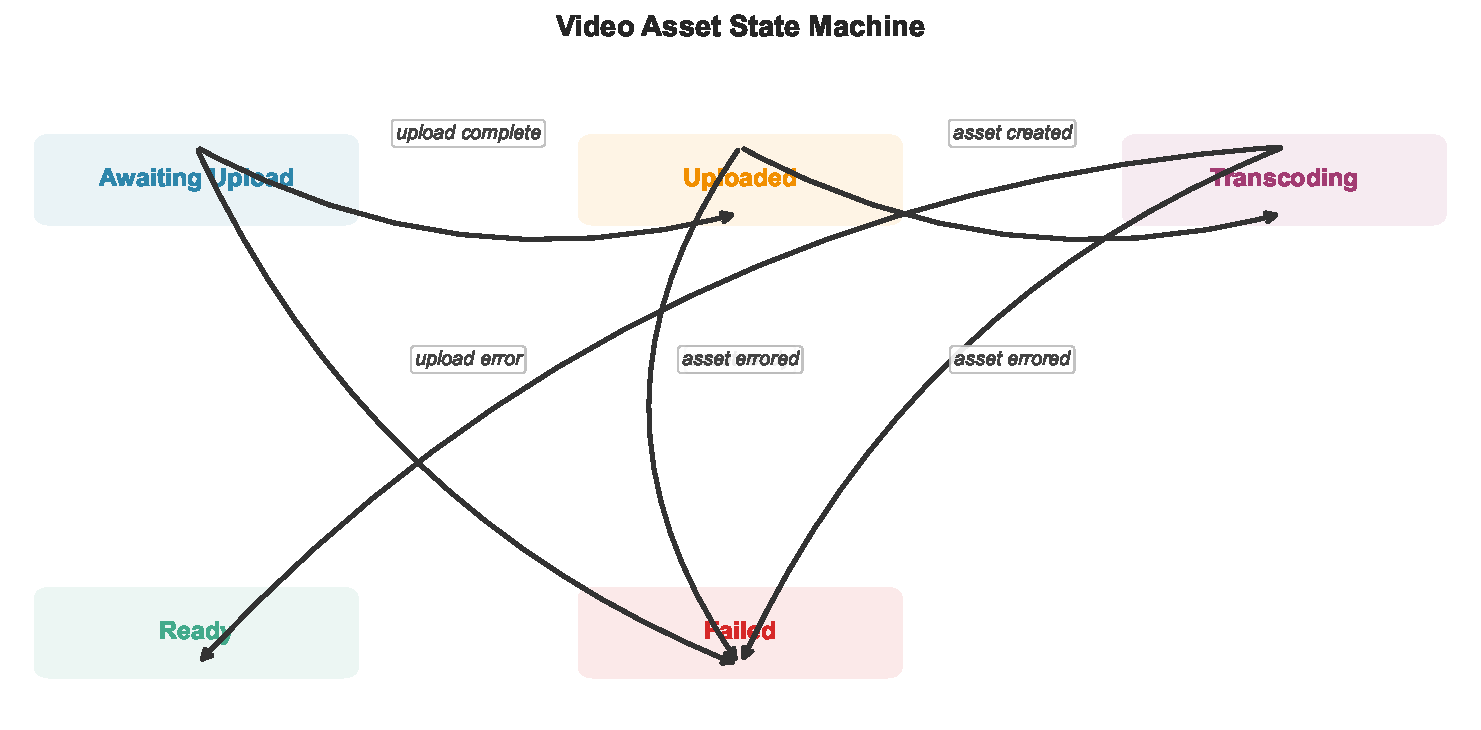
\includegraphics[width=0.75\textwidth]{images/statemachines/video_asset_statemachine.pdf}
  \caption{Video Asset State Machine}
  \label{fig:video-statemachine}
\end{figure}

The lifecycle proceeds as follows:

\begin{enumerate}
  \item \textbf{AWAITING\_UPLOAD.} A lesson is created, and an instructor calls \texttt{POST /instructor/video-assets/upload-url} to request a direct upload URL. The server calls Mux's \texttt{Upload.create()} API, obtains a signed upload URL, and stores the \texttt{upload\_id} in the \texttt{VideoAsset} entity.
  \item \textbf{UPLOADED.} The client PUTs the video file directly to Mux using the signed URL. The server does not proxy the file, avoiding bandwidth costs and latency. The state transitions to UPLOADED once Mux confirms receipt.
  \item \textbf{TRANSCODING.} Mux sends \texttt{video.upload.asset\_created}, indicating that the source file is being transcoded into HLS renditions. The Media module updates the state and creates a \texttt{GenerationJob} in the AI Pipeline module with status QUEUED.
  \item \textbf{READY.} Mux sends \texttt{video.asset.ready} with the playback ID. The Media module stores the playback ID, sets the signed URL expiry policy, and transitions the asset to READY. An outbox event \texttt{VideoReady} is published, triggering the AI pipeline to begin transcript generation.
  \item \textbf{FAILED.} Mux sends \texttt{video.asset.errored} with an error code. The state transitions to FAILED, and the instructor is notified via the Notifications module.
\end{enumerate}

\subsection{Signed Playback URL Generation}

Playback URLs are generated by the backend on request and are not stored directly. When a learner accesses a lesson, the backend verifies that the learner has an active enrollment for the course containing that lesson, then generates a JWT-signed playback URL with a 4-hour expiration:

\begin{lstlisting}[caption=Generating a Signed Mux Playback URL,label=lst:signed-url]
async function getPlaybackUrl(
  learnerId: string, lessonId: string
): Promise<string> {
  const enrollment = await this.enrollmentRepo
    .findActiveByLearnerAndLesson(learnerId, lessonId);
  if (!enrollment)
    throw new ForbiddenException('No active enrollment');

  const lesson = await this.lessonRepo.findByIdOrThrow(lessonId);
  const token = this.muxJwtService.sign({
    sub: learnerId,
    aud: `playback:${lesson.videoAsset.playbackId}`,
    exp: Math.floor(Date.now() / 1000) + 14400, // 4 hours
  });

  return `https://stream.mux.com/${lesson.videoAsset.playbackId}.m3u8?token=${token}`;
}
\end{lstlisting}

This design ensures that: (1) learners cannot share playback URLs beyond the 4-hour window; (2) revoked enrollments are immediately reflected---the next request generates a playback URL only if the enrollment is still active; and (3) unauthorised users never receive a valid playback URL because the authorization check happens server-side before the JWT is signed.

Figure~\ref{fig:seq-video-streaming} illustrates the end-to-end flow. The instructor uploads a video through the Media module, which obtains a Mux upload URL without proxying the file. The client uploads directly to Mux. Asynchronous webhooks drive the state machine: \texttt{video.upload.asset\_created} transitions to UPLOADED and then TRANSCODING; \texttt{video.asset.ready} transitions to READY and stores the playback ID. When a learner later requests the lesson content, the server verifies the learner has an active enrollment, generates a signed JWT playback URL with a 4-hour expiry, and the client streams HLS segments directly from the Mux CDN.

\begin{figure}[H]
  \centering
  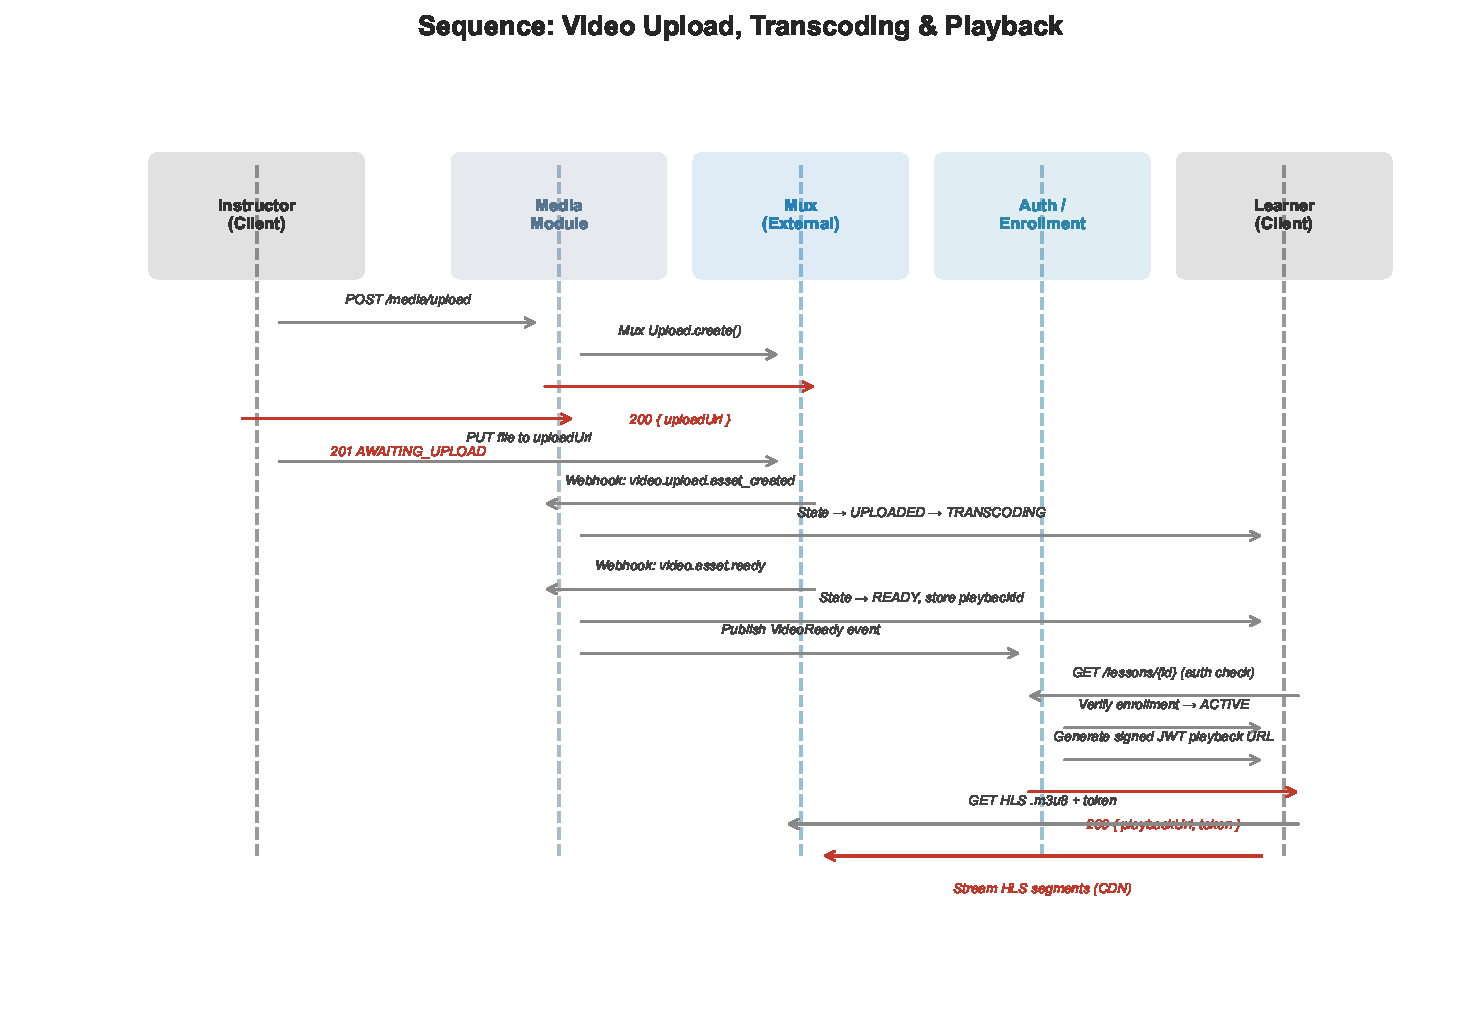
\includegraphics[width=0.85\textwidth]{images/seq_video_streaming.pdf}
  \caption{Sequence Diagram: Video Upload, Transcoding \& Playback}
  \label{fig:seq-video-streaming}
\end{figure}
